\chapter{Sprint 5: Reporting and Analytics Dashboard}

\section{Introduction}

The fifth sprint implements comprehensive reporting and analytics capabilities enabling data-driven decision making through intelligent visualization, flexible filtering, and multi-format export functionality.

Network operations generate massive data volumes across sites, equipment, maintenance activities, incidents, and alerts requiring sophisticated analysis tools. The reporting system aggregates data from multiple modules presenting unified views of network health, operational efficiency, and service quality metrics.

Advanced visualization techniques including interactive charts, trend analysis, and comparative statistics enable stakeholders to identify patterns, detect anomalies, and make informed decisions supporting operational excellence.

\section{Sprint Backlog}

Table \ref{tab:sprint5-backlog} presents the Sprint 5 backlog covering reporting, analytics, and data export functionalities.

\begin{table}[H]
\centering
\scriptsize
\caption{Sprint 5 Backlog - Reporting and Analytics}
\label{tab:sprint5-backlog}
\begin{tabular}{|p{2.8cm}|p{4cm}|p{5cm}|c|c|}
\hline
\textbf{Functionality} & \textbf{User Story} & \textbf{Tasks} & \textbf{Complexity} & \textbf{Hours} \\
\hline
Analytics Dashboard & As a manager, I want comprehensive analytics dashboard for operations overview & Create dashboard layout, aggregate statistics, implement KPIs & High & 8h \\
\hline
Interactive Charts & As an engineer, I want interactive charts for data visualization & Implement chart components, add filtering, enable drill-down & High & 7h \\
\hline
Custom Reports & As a manager, I want to generate custom reports with date ranges & Create report builder, implement date filters with presets & Medium & 6h \\
\hline
Breakdown Analysis & As an engineer, I want detailed breakdown analysis with metrics & Calculate MTTR/MTBF, show impact analysis & Medium & 6h \\
\hline
Export to CSV & As a manager, I want to export reports to CSV & Implement CSV generation, handle large datasets & Medium & 5h \\
\hline
Export to PDF & As an admin, I want to export reports to PDF & Implement PDF with jsPDF, add progress tracking & High & 7h \\
\hline
Performance KPIs & As a manager, I want to view key performance indicators & Calculate uptime, response time, efficiency metrics & Medium & 5h \\
\hline
Date Range Filter & As a user, I want to filter reports by date period & Implement date picker with presets and custom range & Medium & 6h \\
\hline
\multicolumn{4}{|r|}{\textbf{Total:}} & \textbf{50h} \\
\hline
\end{tabular}
\end{table}

\section{Class Diagram}

Figure \ref{fig:sprint5-class} illustrates the reporting system architecture.

\begin{figure}[H]
\centering
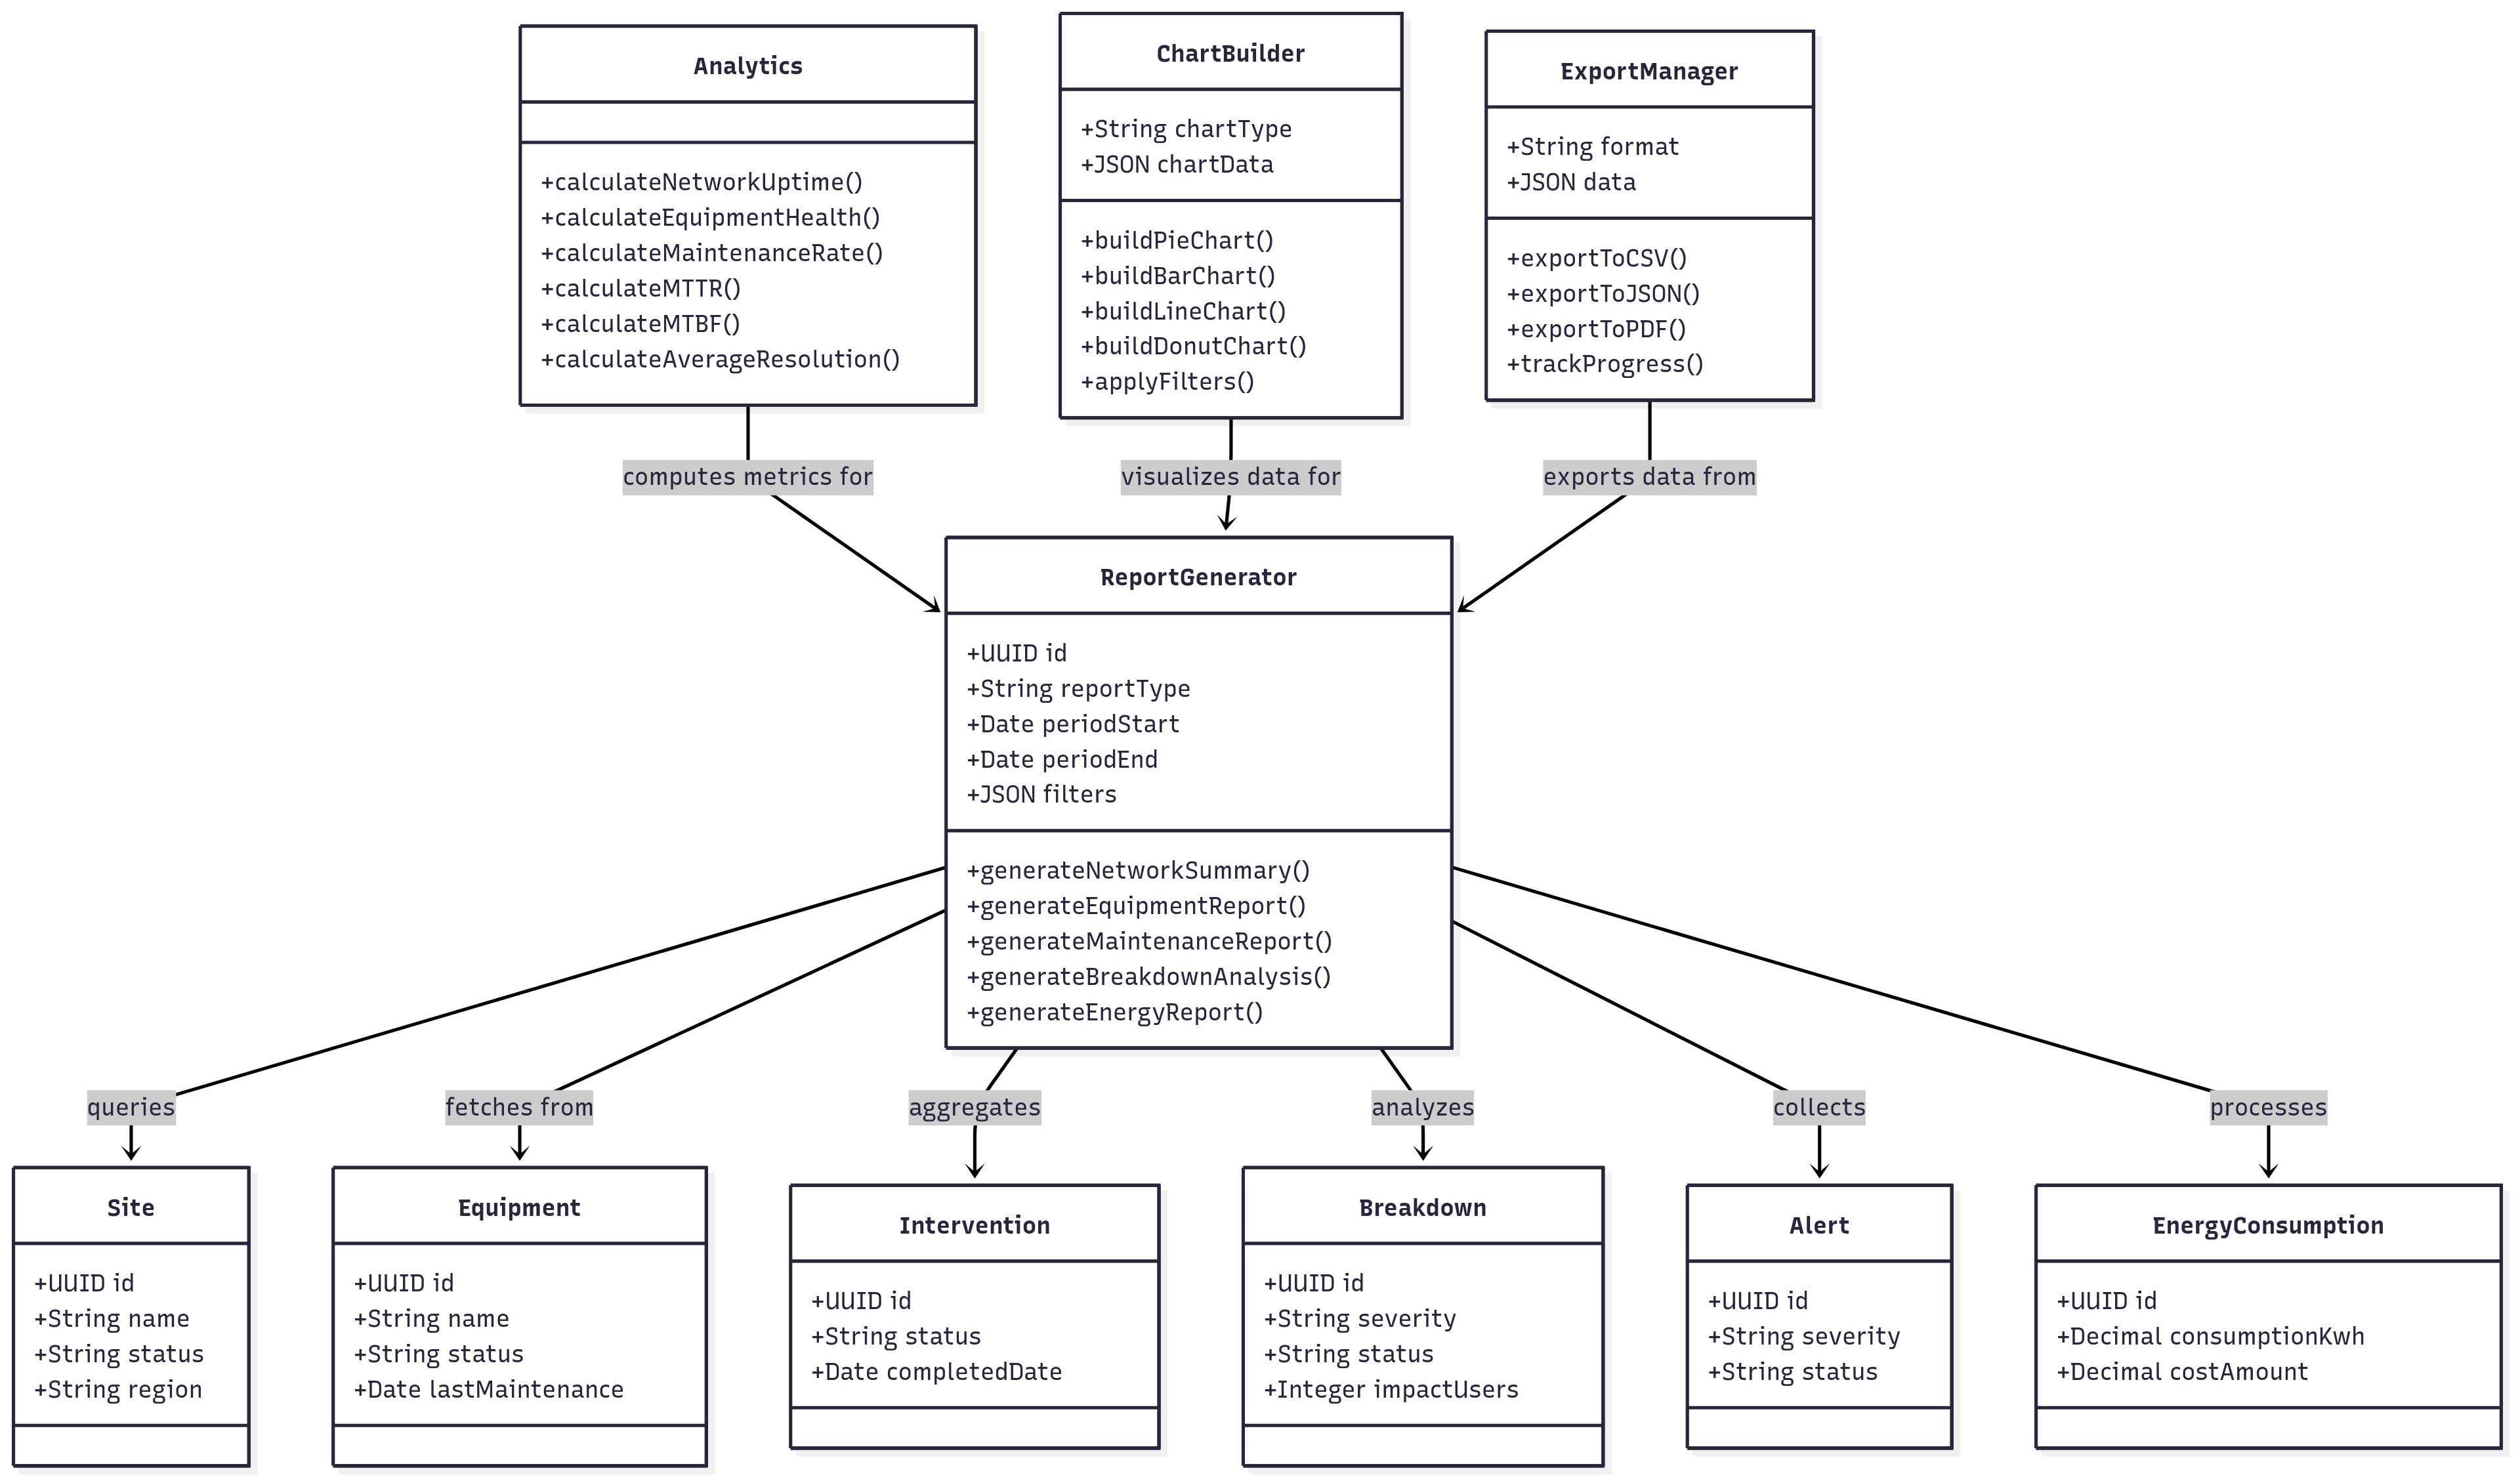
\includegraphics[width=0.7\textwidth]{img/chap_07/sprint5_class_diagram.png}
\caption{Class diagram for reporting and analytics system}
\label{fig:sprint5-class}
\end{figure}

The reporting architecture aggregates data from \texttt{Site}, \texttt{Equipment}, \texttt{Intervention}, \texttt{Breakdown}, \texttt{Alert}, and \texttt{EnergyConsumption} entities.

The \texttt{ReportGenerator} class creates various report types including network summary, equipment status, maintenance history, and breakdown analysis.

The \texttt{Analytics} class calculates KPIs including network uptime, MTTR, MTBF, and response time metrics.

The \texttt{ChartBuilder} transforms data into visualization formats supporting line, bar, pie, and area charts.

The \texttt{ExportManager} handles data export in CSV, JSON, and PDF formats.

\section{Use Case Diagram}

Figure \ref{fig:sprint5-usecase} presents the use case diagram with role-based inheritance hierarchy.

\begin{figure}[H]
\centering
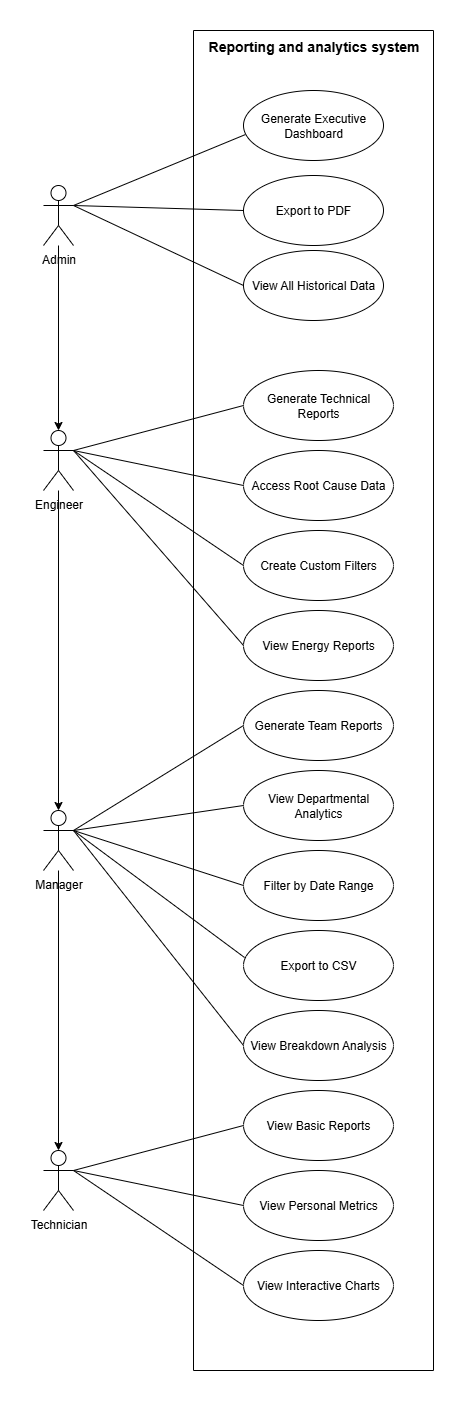
\includegraphics[width=0.7\textwidth]{img/chap_07/sprint5_usecase_diagram.png}
\caption{Use case diagram with role inheritance for Sprint 5}
\label{fig:sprint5-usecase}
\end{figure}

\textbf{Field Technicians} access basic reports and personal performance metrics.

\textbf{Managers} inherit technician capabilities plus team reports, departmental analytics, and CSV export.

\textbf{Network Engineers} add technical reports, root cause analysis, and custom filtering.

\textbf{Administrators} possess all privileges plus executive dashboards, PDF export, and report scheduling.

\section{Use Case Permissions Table}

Table \ref{tab:sprint5-permissions} details the permission matrix by role.

\begin{table}[H]
\centering
\scriptsize
\caption{Sprint 5 Use Case Permissions by Role}
\label{tab:sprint5-permissions}
\begin{tabular}{|p{5.5cm}|c|c|c|c|}
\hline
\textbf{Use Case} & \textbf{Technician} & \textbf{Manager} & \textbf{Engineer} & \textbf{Admin} \\
\hline
View Basic Reports & Yes & Yes & Yes & Yes \\
\hline
View Personal Metrics & Yes & Yes & Yes & Yes \\
\hline
View Interactive Charts & Yes & Yes & Yes & Yes \\
\hline
Generate Team Reports & No & Yes & Yes & Yes \\
\hline
View Departmental Analytics & No & Yes & Yes & Yes \\
\hline
Compare Period Performance & No & Yes & Yes & Yes \\
\hline
Export to CSV & No & Yes & Yes & Yes \\
\hline
View Breakdown Analysis & No & Yes & Yes & Yes \\
\hline
Generate Technical Reports & No & No & Yes & Yes \\
\hline
Access Root Cause Data & No & No & Yes & Yes \\
\hline
Create Custom Filters & No & No & Yes & Yes \\
\hline
Generate Executive Dashboard & No & No & No & Yes \\
\hline
Export to PDF & No & No & No & Yes \\
\hline
Configure Report Templates & No & No & No & Yes \\
\hline
\end{tabular}
\end{table}

\section{Use Case Description}

Table \ref{tab:sprint5-usecase-detail} describes the "Generate Report" use case.

\begin{table}[H]
\centering
\scriptsize
\caption{Detailed Description - Generate Report Use Case}
\label{tab:sprint5-usecase-detail}
\begin{tabular}{|p{3cm}|p{10.5cm}|}
\hline
\textbf{Element} & \textbf{Description} \\
\hline
\textbf{Use Case Name} & Generate Report \\
\hline
\textbf{Actor} & Network Engineer, Manager, Administrator \\
\hline
\textbf{Description} & Generate comprehensive reports aggregating operational data across selected time periods with customizable filtering and visualization \\
\hline
\textbf{Preconditions} & User authenticated; Historical data available; Aggregation services operational \\
\hline
\textbf{Postconditions} & Report generated and displayed; Export options available; Activity logged \\
\hline
\textbf{Main Flow} & 1. Navigate to reports dashboard \newline 2. Select report type \newline 3. Set date range using presets or custom selection \newline 4. Apply optional filters \newline 5. Click "Generate Report" \newline 6. System validates parameters \newline 7. System aggregates data \newline 8. System calculates metrics \newline 9. System generates visualizations \newline 10. Display complete report \newline 11. Enable export options \\
\hline
\textbf{Alternative Flow} & \textbf{A1 - PDF Export:} User selects "Export PDF", system shows progress tracking, generates PDF with staging, triggers download when complete \\
\hline
\textbf{Exception Flow} & \textbf{E1 - Insufficient Data:} Display warning with alternative suggestions \newline \textbf{E2 - Large Dataset:} Initiate background processing with email notification \newline \textbf{E3 - Export Failure:} Log error and offer retry options \\
\hline
\end{tabular}
\end{table}

\section{Sequence Diagrams}

\subsection{Generate Report Sequence}

Figure \ref{fig:sprint5-seq1} shows report generation with data aggregation.

\begin{figure}[H]
\centering
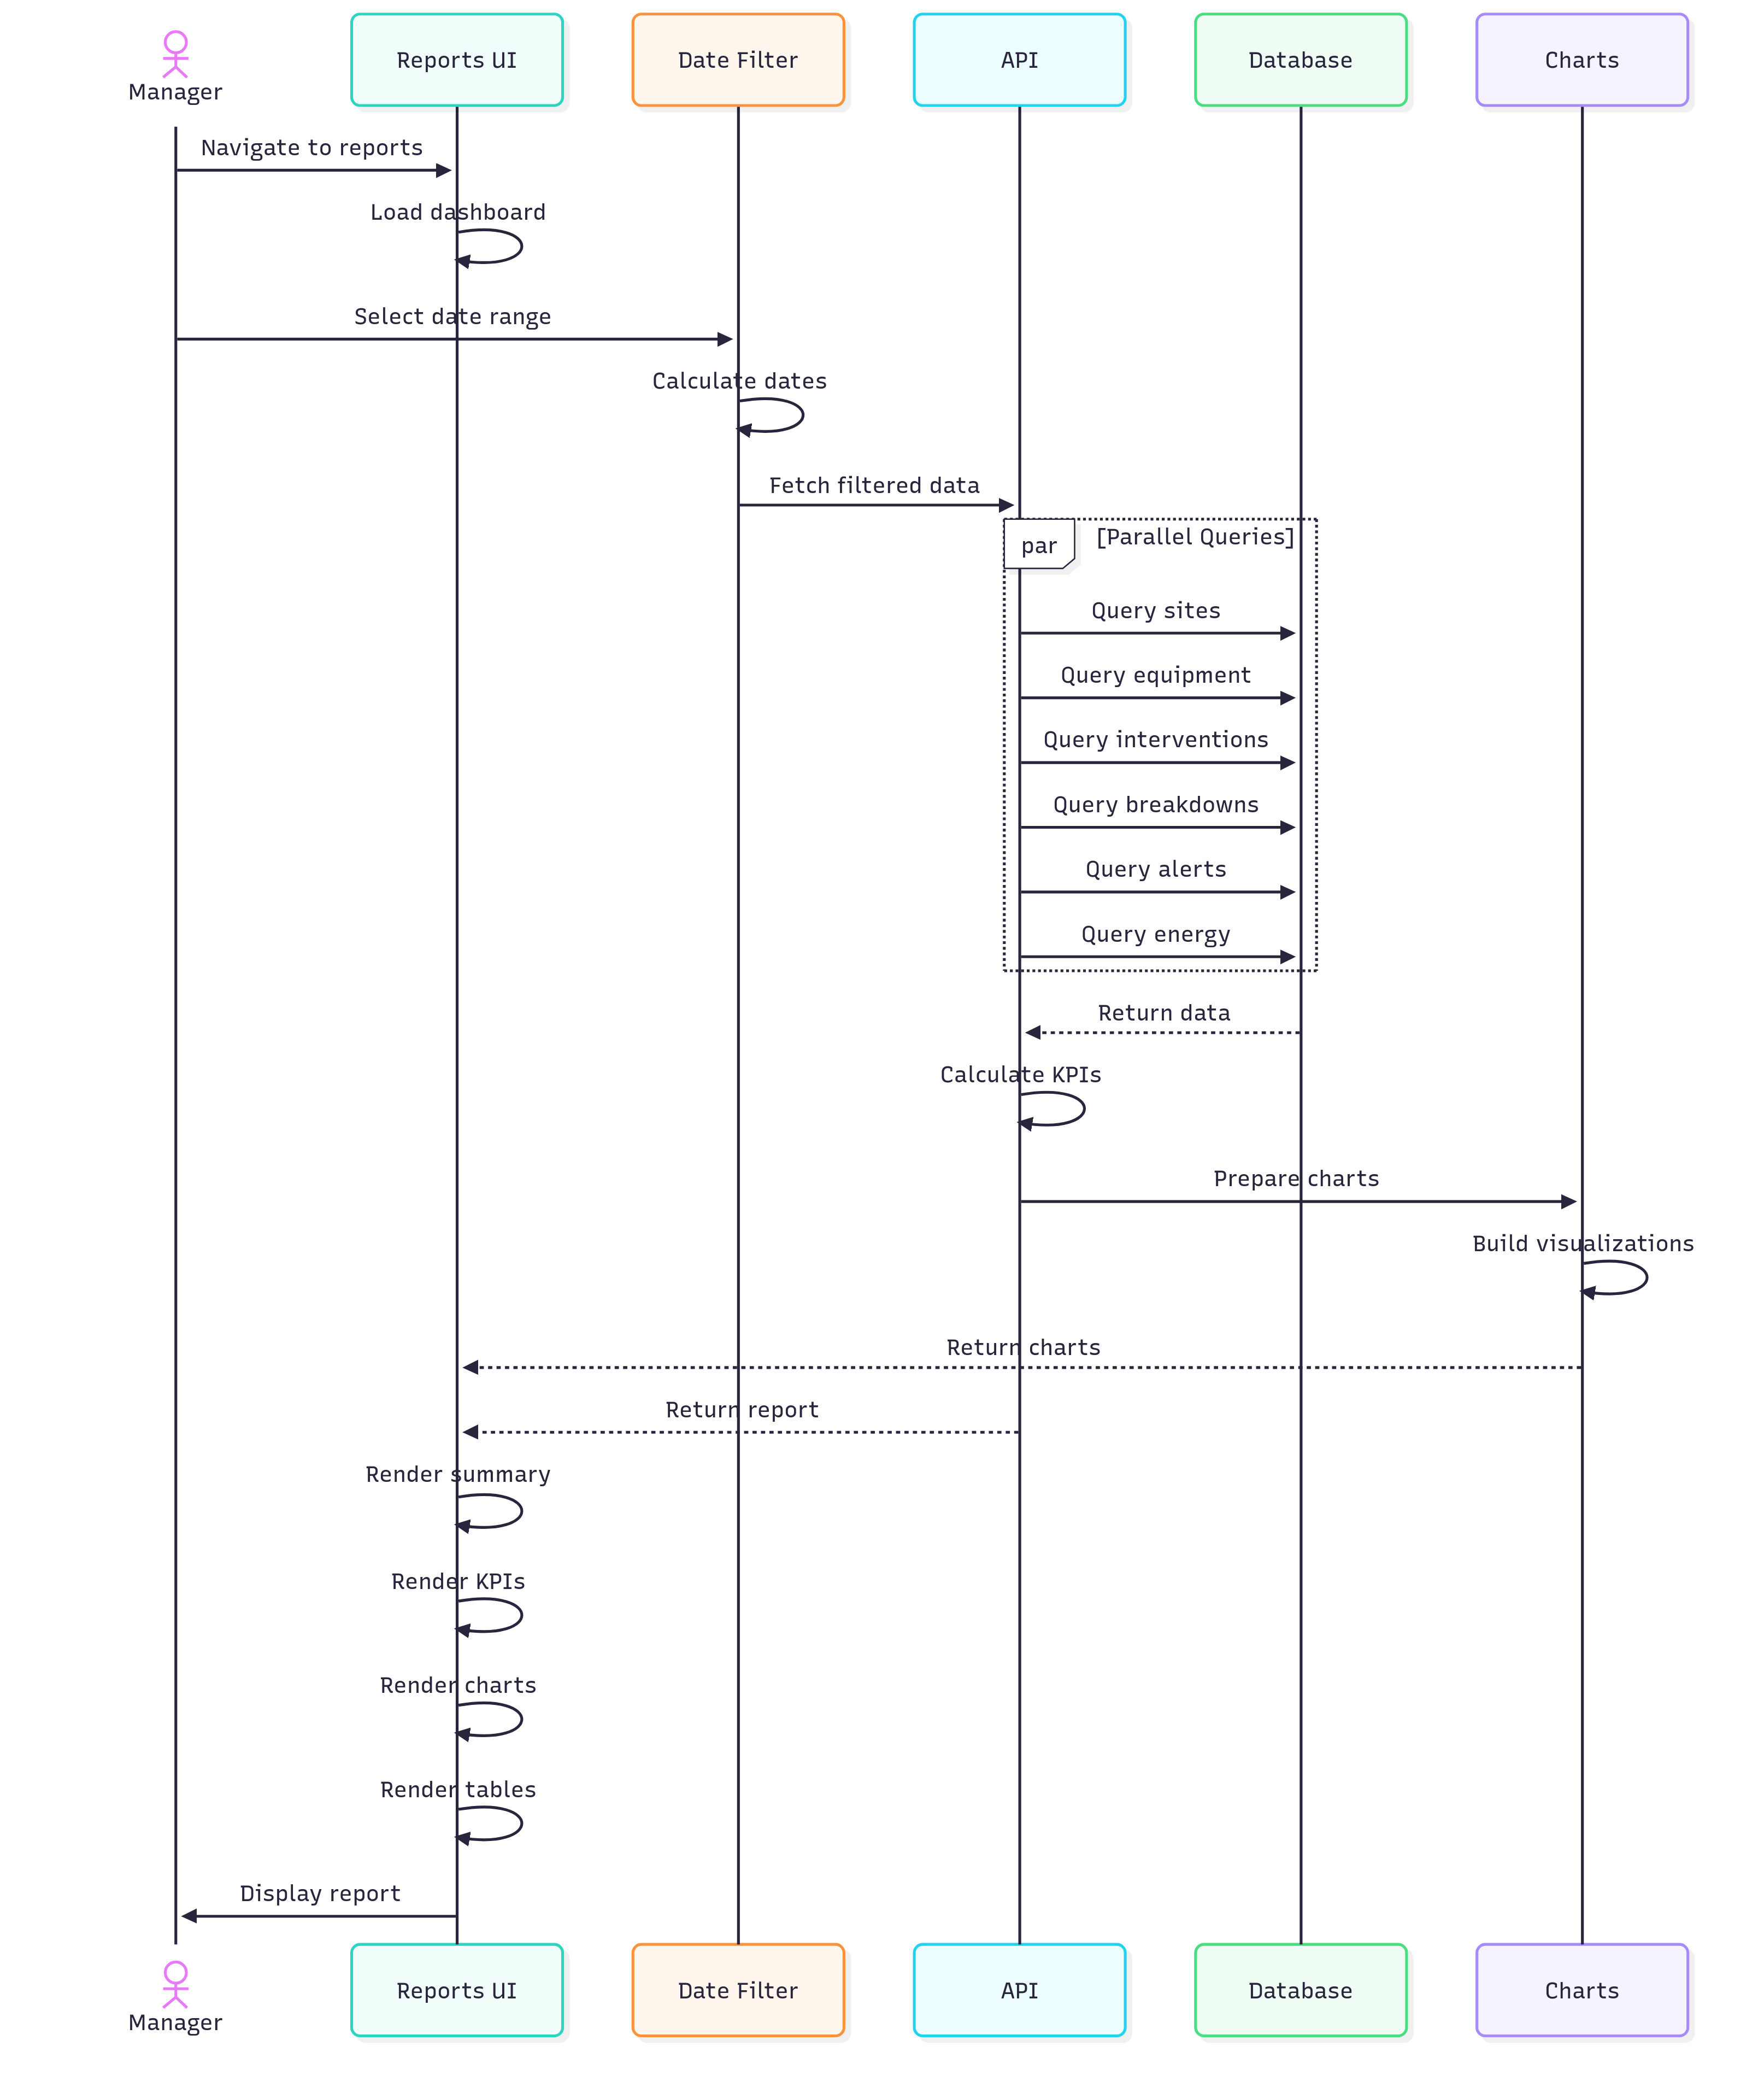
\includegraphics[width=0.7\textwidth]{img/chap_07/sprint5_sequence_report.png}
\caption{Sequence diagram for generating analytical reports}
\label{fig:sprint5-seq1}
\end{figure}

\subsection{Export Data Sequence}

Figure \ref{fig:sprint5-seq2} illustrates data export workflow to CSV, JSON, and PDF.

\begin{figure}[H]
\centering
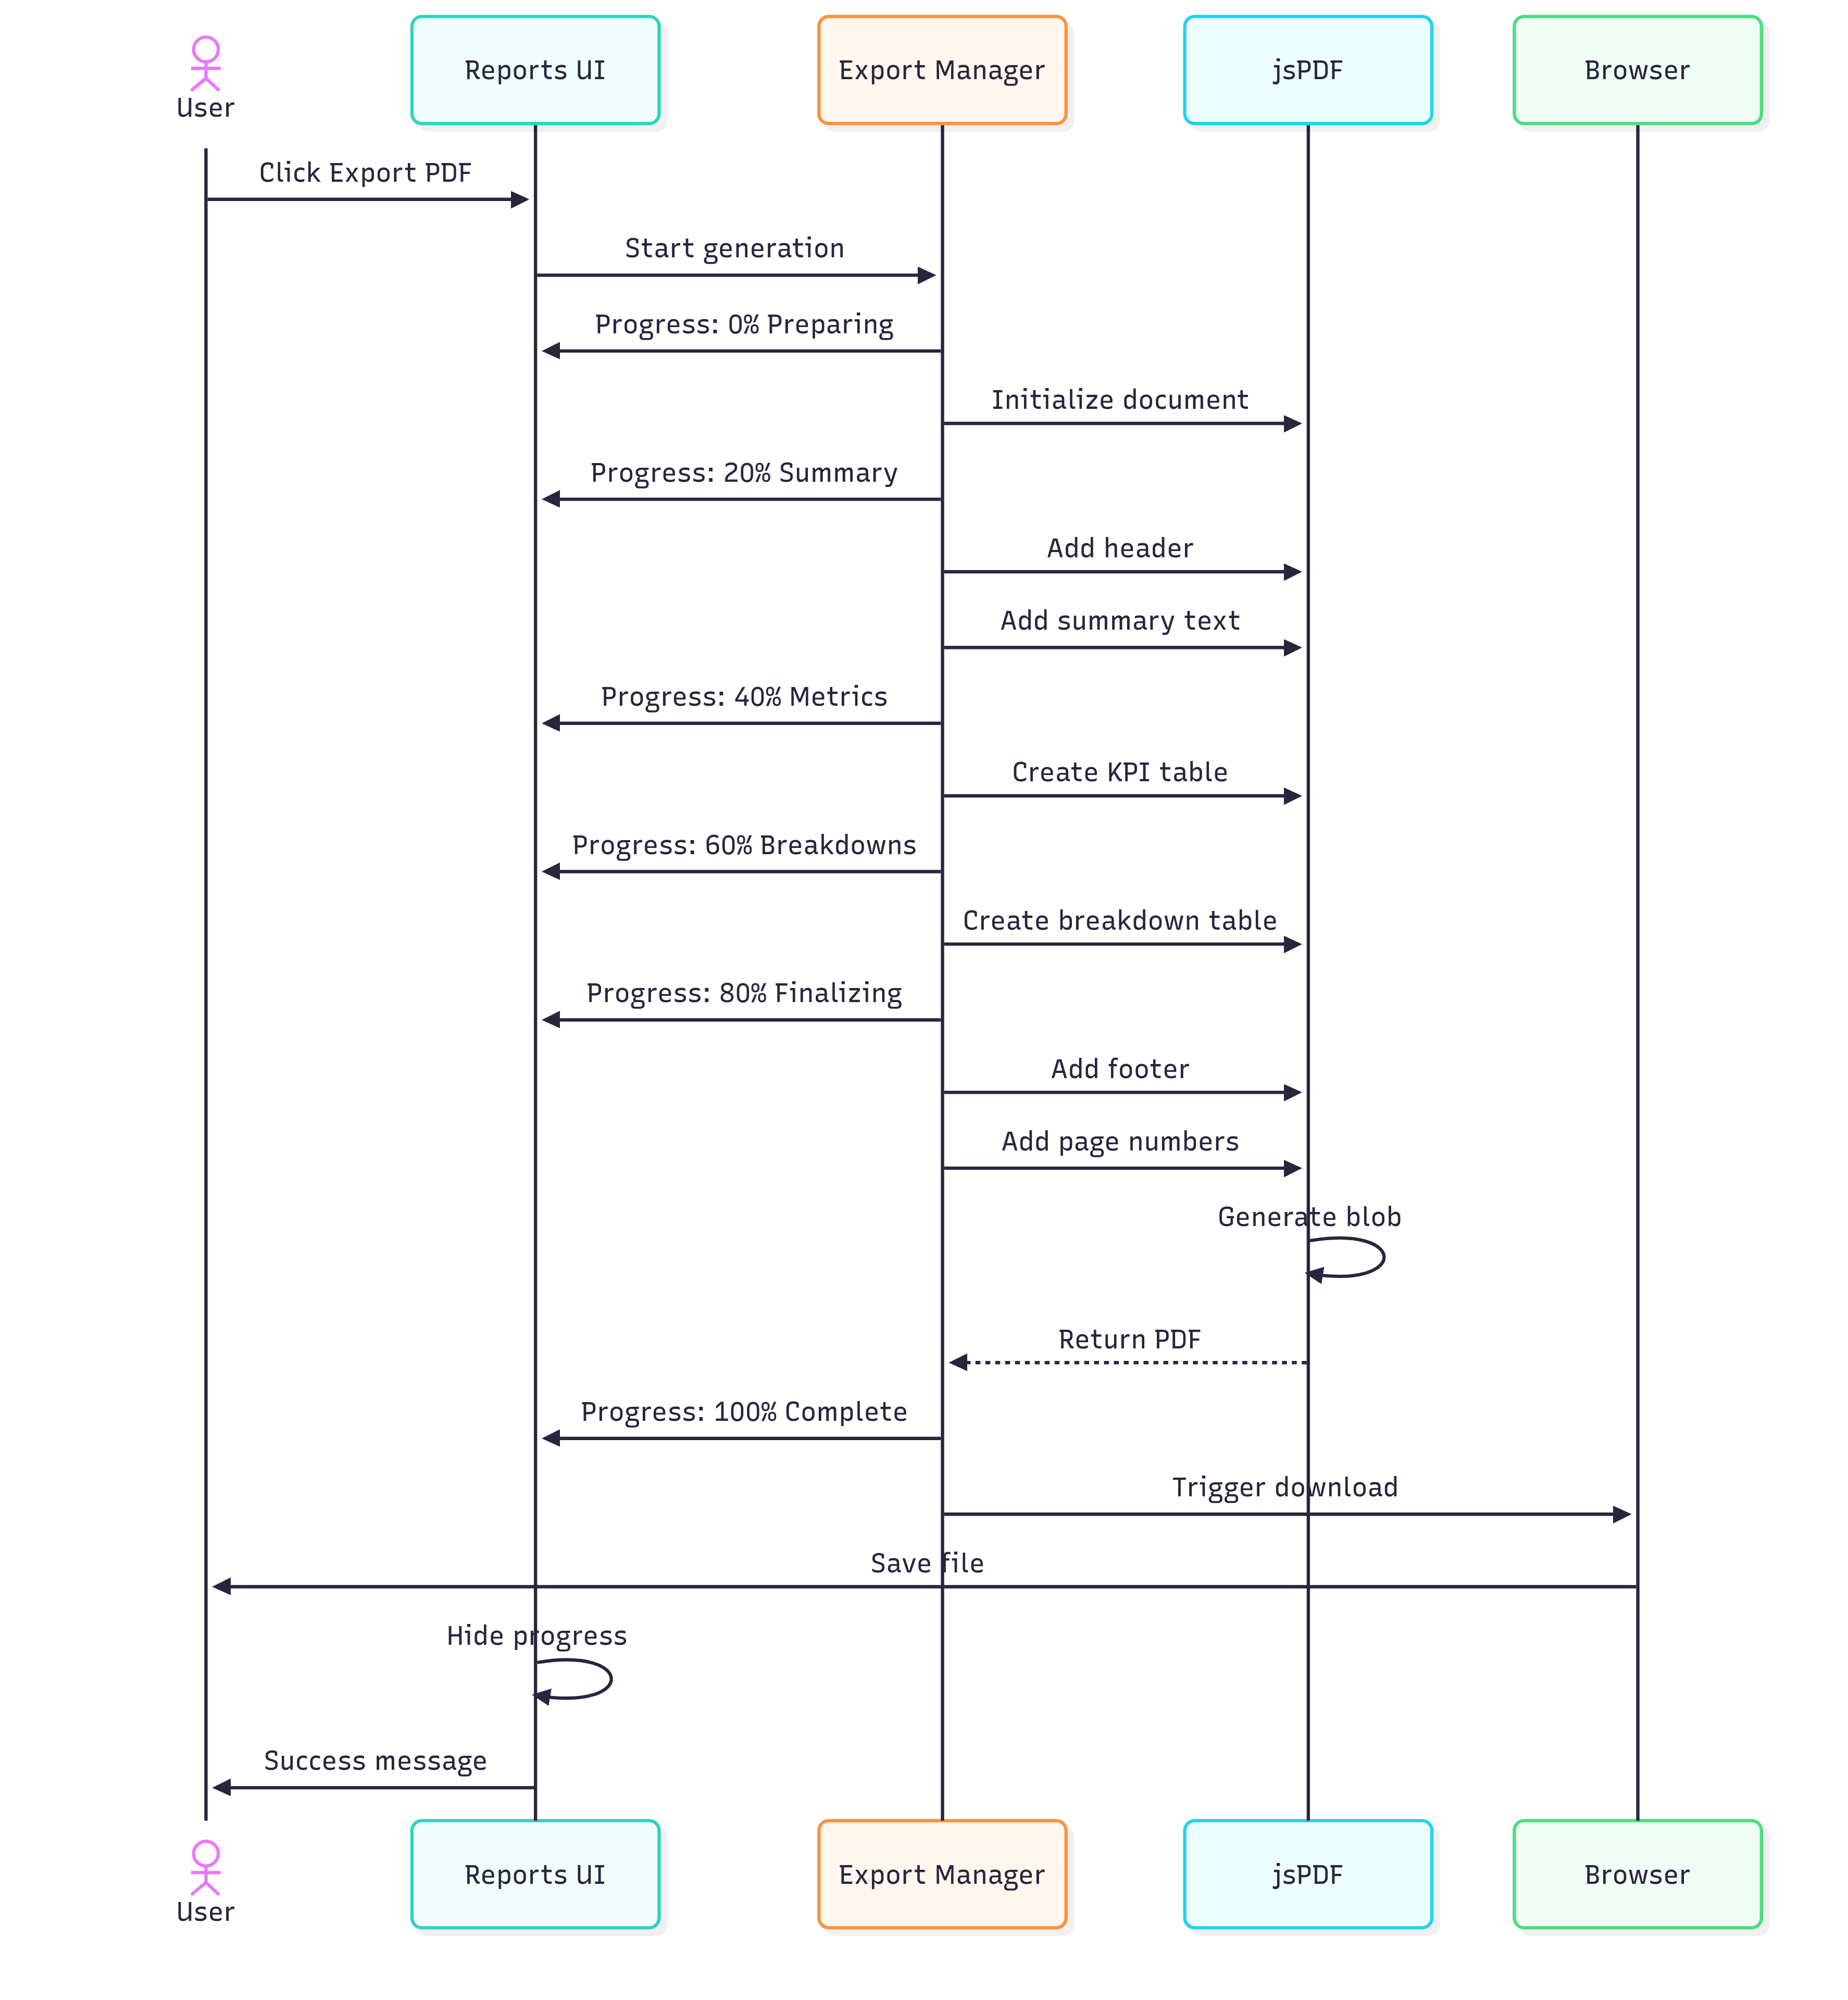
\includegraphics[width=0.7\textwidth]{img/chap_07/sprint5_sequence_export.png}
\caption{Sequence diagram for exporting report data}
\label{fig:sprint5-seq2}
\end{figure}

\section{Implementation}

\subsection{Analytics Dashboard Overview}

Figure \ref{fig:sprint5-impl1} shows the main analytics dashboard.

\begin{figure}[H]
\centering
\fbox{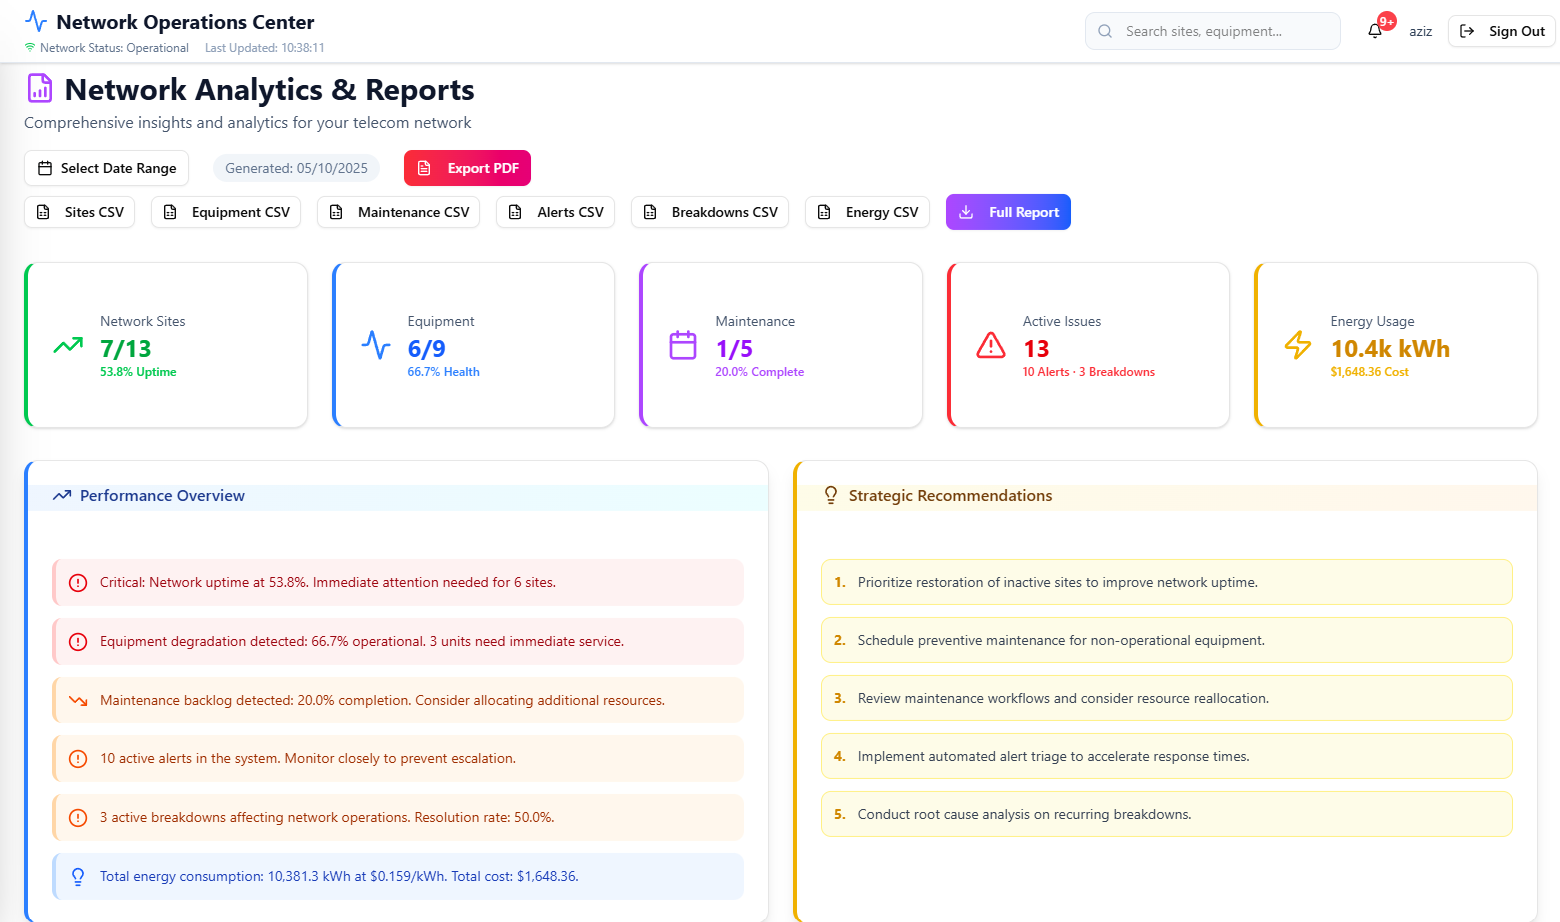
\includegraphics[width=0.70\textwidth]{img/chap_07/screenshot_analytics_dashboard.png}}
\caption{Analytics dashboard with KPIs and intelligent insights}
\label{fig:sprint5-impl1}
\end{figure}

The dashboard displays critical metrics including network uptime, equipment health, maintenance completion rate, and breakdown resolution efficiency.

The intelligent summary section provides narrative insights with color-coded status indicators.

Quick insight cards show sites count, online percentage, equipment total, and active alerts.

\subsection{Interactive Charts}

Figure \ref{fig:sprint5-impl2} displays interactive charts.

\begin{figure}[H]
\centering
\fbox{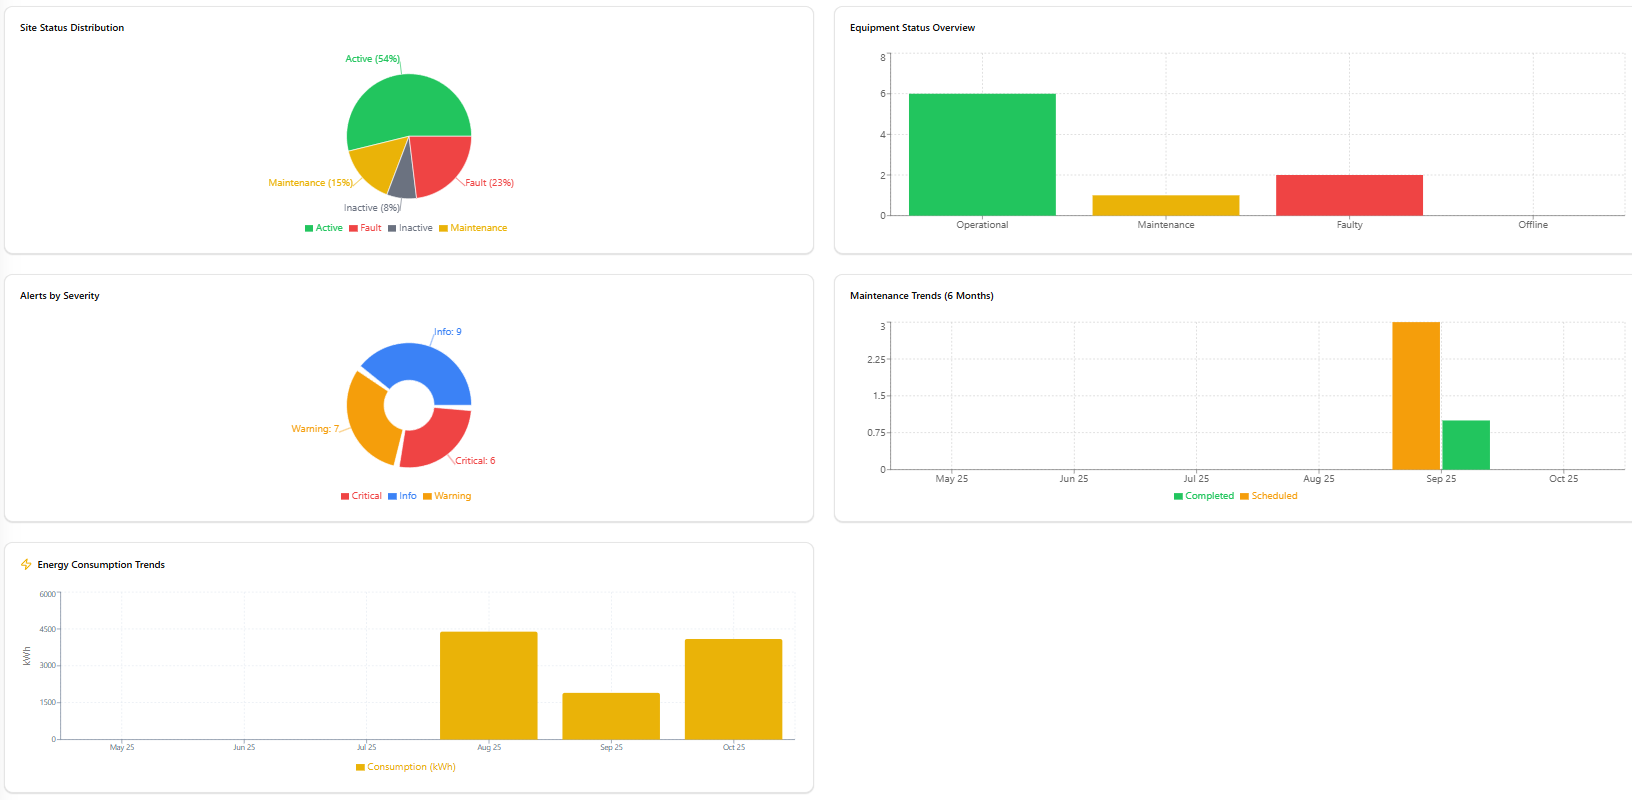
\includegraphics[width=0.70\textwidth]{img/chap_07/screenshot_charts_visualization.png}}
\caption{Interactive charts showing operational trends}
\label{fig:sprint5-impl2}
\end{figure}

The system uses Recharts library with pie charts for status distribution, bar charts for comparisons, and line charts for trends.

Interactive features enable filtering, drill-down, tooltips, and legend interactions.

Responsive design ensures accessibility across devices.

\subsection{Breakdown Analysis}

Figure \ref{fig:sprint5-impl3} presents breakdown analysis.

\begin{figure}[H]
\centering
\fbox{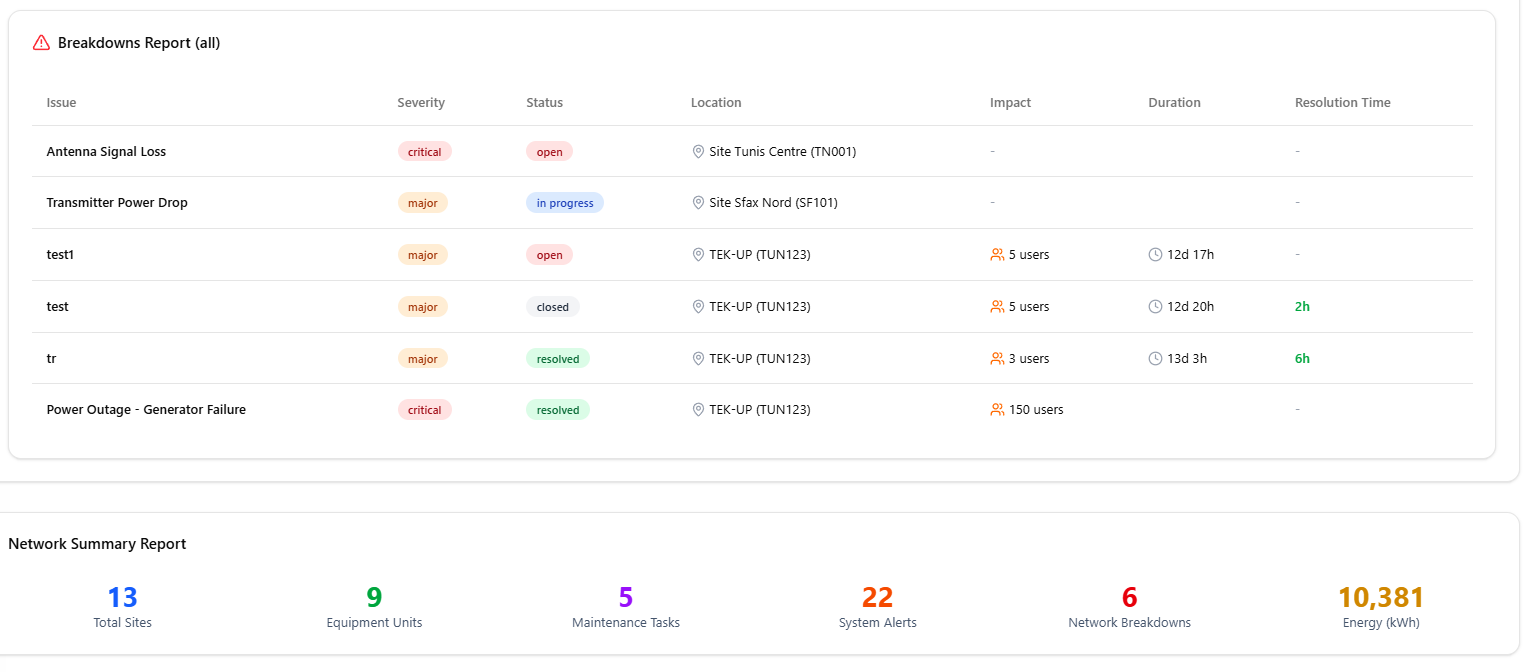
\includegraphics[width=0.7\textwidth]{img/chap_07/screenshot_breakdown_analysis.png}}
\caption{Breakdown analysis with performance metrics}
\label{fig:sprint5-impl3}
\end{figure}

The interface shows total breakdowns, active issues, critical count, resolution status, and impact statistics.

The table displays descriptions, severity, status, locations, user impact, and resolution times.

Color-coded badges enable quick priority identification.

\subsection{Date Range Filter}

Figure \ref{fig:sprint5-impl4} shows the date filter.

\begin{figure}[H]
\centering
\fbox{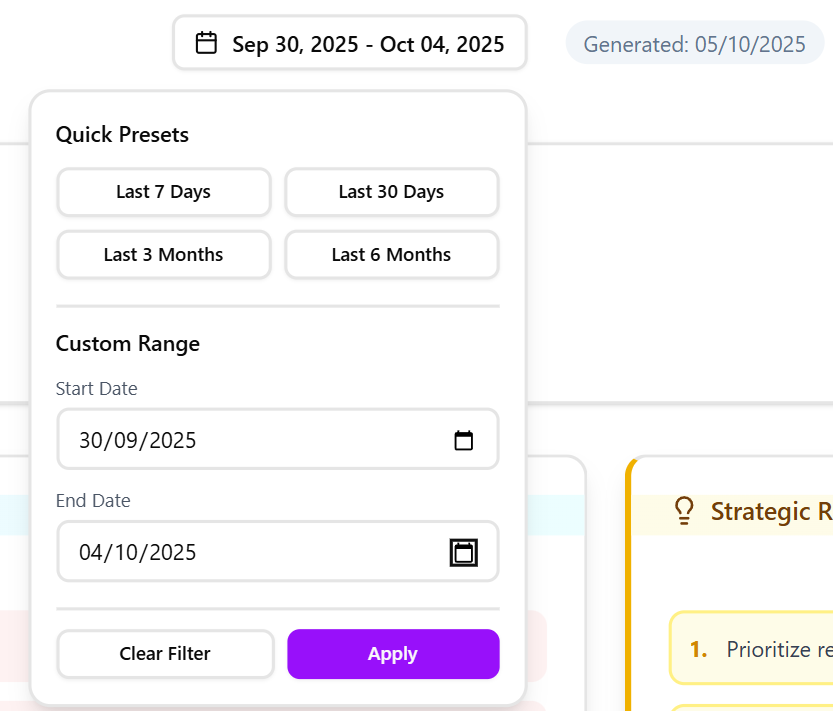
\includegraphics[width=0.70\textwidth]{img/chap_07/screenshot_date_filter..png}}
\caption{Date range filter with quick presets}
\label{fig:sprint5-impl4}
\end{figure}

Quick presets include Last 7 Days, Last 30 Days, Last 3 Months, and Last 6 Months.

Custom selection allows precise start and end dates.

Real-time filtering applies across all dashboard components.

\subsection{PDF Export with Progress}

Figure \ref{fig:sprint5-impl5} displays PDF export functionality.

\begin{figure}[H]
\centering
\fbox{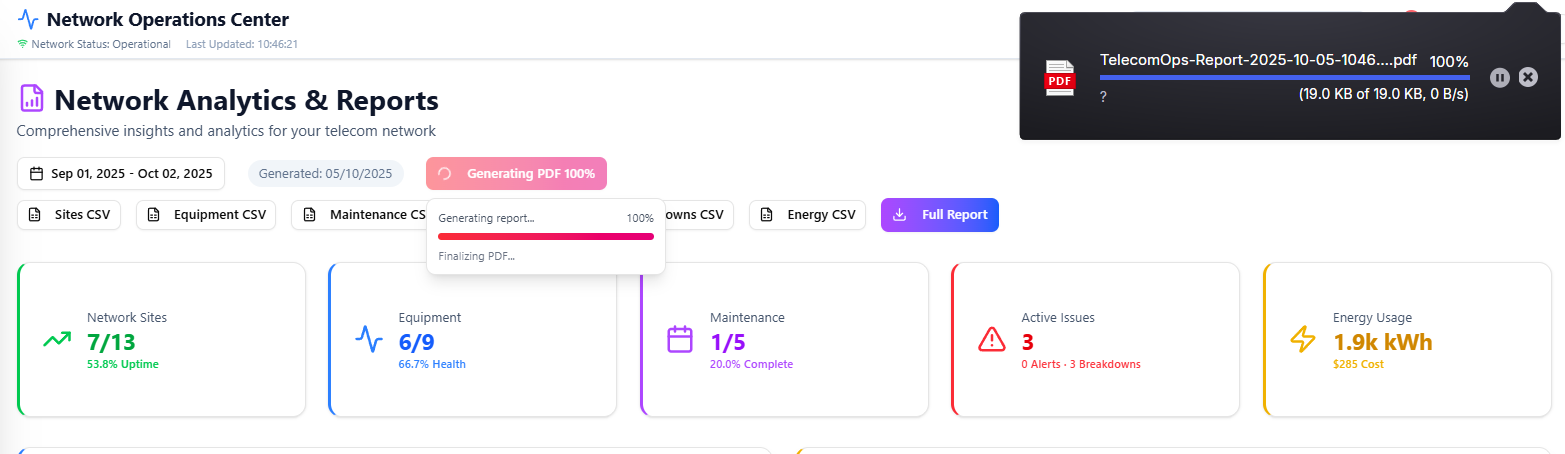
\includegraphics[width=0.70\textwidth]{img/chap_07/screenshot_pdf_export.png}}
\caption{PDF export with progress tracking}
\label{fig:sprint5-impl5}
\end{figure}

The system uses jsPDF for client-side generation with executive summary, KPIs table, breakdown analysis, and branding.

Progress tracking shows five stages: preparation, summary, metrics, breakdowns, and finalization.

Visual progress bar displays 0-100 percent with status messages.

\subsection{Generated PDF Sample}

Figure \ref{fig:sprint5-impl6} shows a generated PDF report.

\begin{figure}[H]
\centering
\fbox{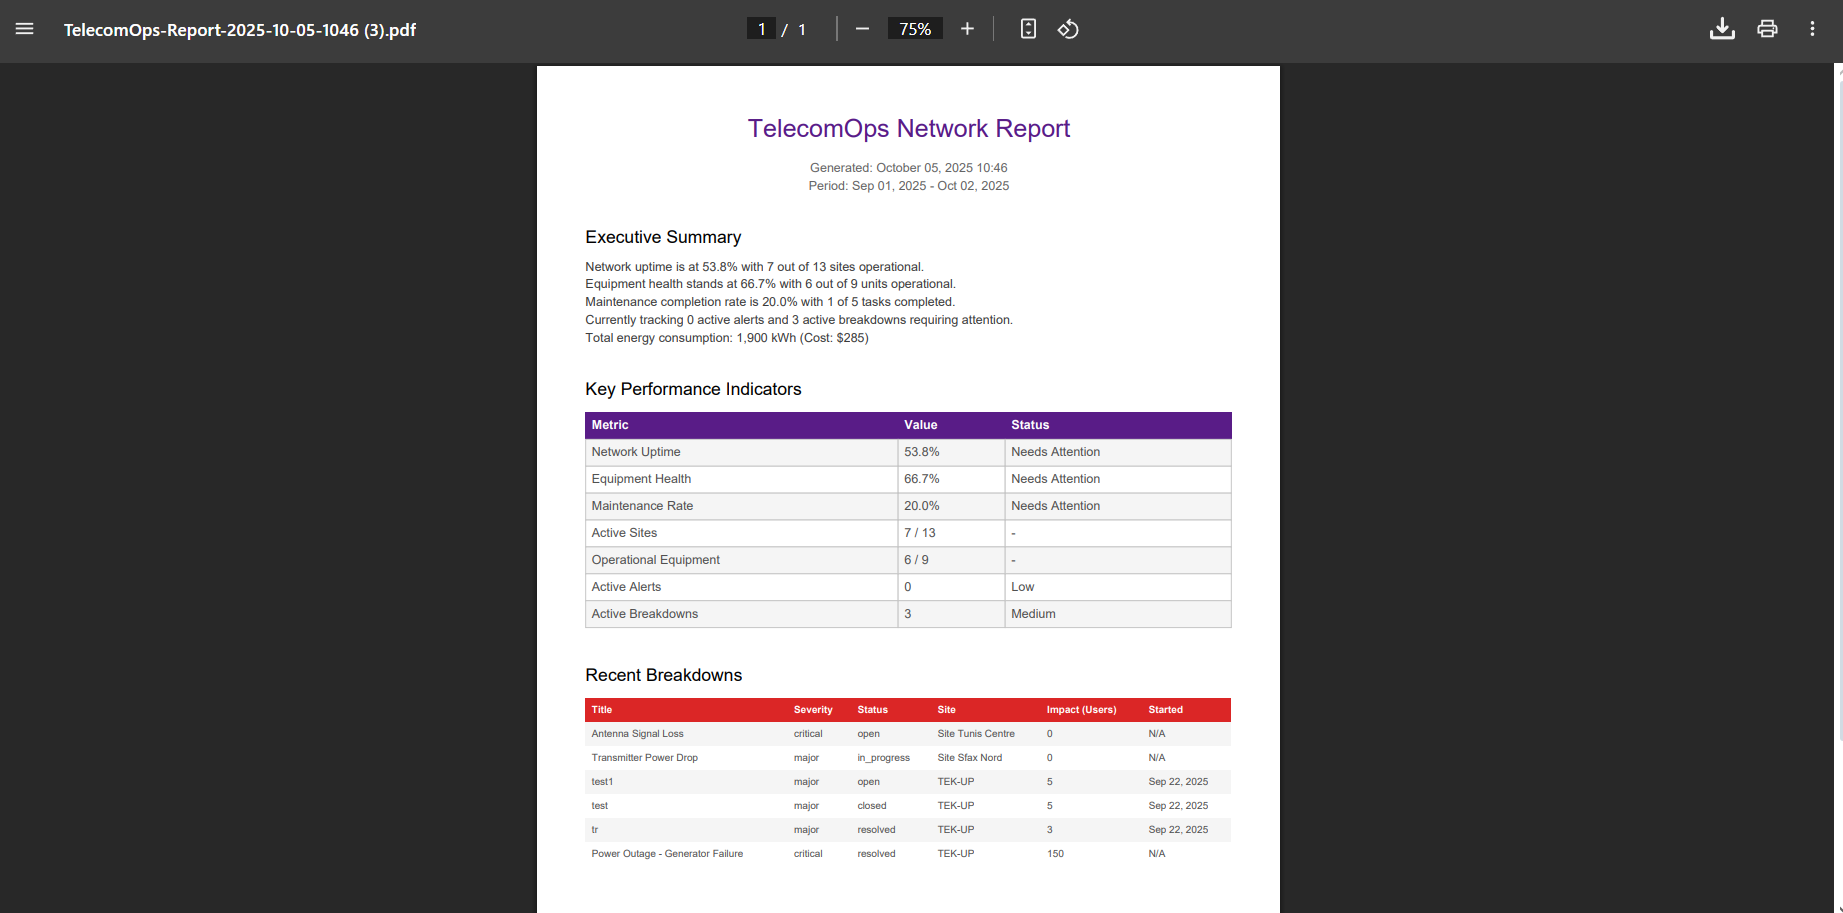
\includegraphics[width=0.70\textwidth]{img/chap_07/screenshot_pdf_sample.png}}
\caption{Generated PDF with summary and metrics}
\label{fig:sprint5-impl6}
\end{figure}

The PDF includes header with timestamp, executive summary, KPIs table, and breakdown details.

Consistent branding with footer and page numbers supports multi-page reports.

\section{Technical Challenges and Solutions}

\subsection{Large Dataset Performance}

\textbf{Challenge:} Generating reports from extensive historical data required query optimization, pagination, memory management, and responsive UX.

\textbf{Solution:} Implemented materialized views for pre-calculated metrics and compound indexes for faster joins.

Application-level optimization uses incremental loading, lazy chart rendering, and virtual scrolling.

Large datasets trigger background processing with email notification and download links.

\subsection{Client-Side PDF Generation}

\textbf{Challenge:} Browser PDF generation required managing memory constraints, formatting tables, handling UTF-8 text, and providing progress feedback.

\textbf{Solution:} Implemented jsPDF with staged generation and progress tracking.

Table formatting uses autoTable plugin for proper sizing and text wrapping.

UTF-8 encoding supports multilingual content with memory-optimized batching.

\subsection{Real-Time Updates}

\textbf{Challenge:} Maintaining dashboard accuracy required efficient change detection, update frequency management, and concurrent session handling.

\textbf{Solution:} Hybrid strategy combines Supabase subscriptions for critical data with intelligent polling for aggregated stats.

React Query implements background refetching and optimistic updates.

Components use memo hooks and batched updates to reduce re-renders.

\section{Testing and Validation}

\subsection{Functional Testing}

Functional testing verified all reporting features across various scenarios.

Report generation validated network summary, equipment status, maintenance history, and breakdown analysis.

Chart rendering confirmed correct visualization across data distributions.

Export functionality validated CSV, JSON, and PDF formats with proper encoding.

\subsection{Integration Testing}

Integration testing ensured proper module integration.

Data sources validated correct aggregation from sites, equipment, interventions, breakdowns, and alerts tables.

Authorization verified role-based access for technicians, managers, engineers, and administrators.

Export integration confirmed compatibility with external tools and PDF readers.

\subsection{User Acceptance Testing}

Tunisia Telecom staff tested reporting in realistic scenarios.

Management appreciated clear KPIs, trend visualization, and actionable insights.

Engineers valued breakdown analysis, maintenance trends, and custom filtering.

Field supervisors confirmed mobile usability and offline caching.

Overall feedback highlighted value from automated metrics replacing manual compilation.

\section{Conclusion}

Sprint 5 delivered comprehensive reporting and analytics transforming operational data into actionable intelligence.

The analytics dashboard provides unified visibility aggregating metrics from all system modules through intuitive visualizations and customizable reports.

Interactive charting enables trend identification and comparative analysis supporting tactical and strategic decisions.

Date range filtering with presets and custom selection enables flexible period analysis across all dashboard components.

Export functionality supporting CSV, JSON, and PDF enables external integration and stakeholder distribution. PDF generation with progress tracking provides professional reports with branding and formatting.

Technical challenges around performance, PDF generation, and real-time updates were resolved through optimization strategies and hybrid approaches.

Testing validated functional correctness, integration quality, and strong user acceptance.

Sprint 5 establishes foundation for advanced analytics including predictive maintenance, anomaly detection, and automated insight generation supporting Tunisia Telecom's operational excellence objectives.